\chapter{Introduction}
\label{cha:introduction}
% Intro should be readable to a non expert

\section{Goal}

In many natural complex systems, learning is a key process that allows the
system to adapt and evolve over time. In this thesis, we explore the use of
complex systems as a framework for studying learning and adaptation in natural
and artificial systems. The aim of this thesis is to develop methods to study
and use computations that take place in complex dynamical systems to eventually
create learning algorithms that require limited to no supervision. This
objective is broken down into the following subgoals:

\begin{enumerate}
  \item Identify complex dynamical systems with the potential to exhibit
        emergent open-ended growth of complexity and evolutionary-like
        properties. There are many ways to define complex systems, and as
        illustrated in Figure \ref{fig:comparison_ca}, some may exhibit more
        interesting and promising behaviors than others. Interesting systems,
        such as the cellular automaton (CA) in Figure \ref{fig:structured_sys}
        may not have the same likelihood of being found depending on how the
        search space is defined. The work presented in Chapter
        \ref{cha:meas-compl-evolv} aims at constructing a metric of complexity
        that can help in the identification of interestingly behaving complex
        dynamical systems.
\begin{figure}[htbp]
  \centering
\begin{subfigure}[b]{.4\linewidth}
  \centering
  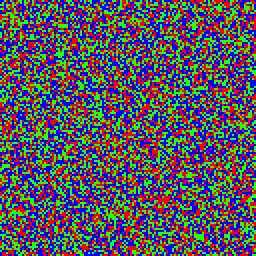
\includegraphics[width=\linewidth]{figures/disord2.png}
  \caption{A disordered \acl{CA}.}
 \label{fig:disordered_sys}
\end{subfigure}
\hspace{30pt}
\begin{subfigure}[b]{.4\linewidth}
  \centering
  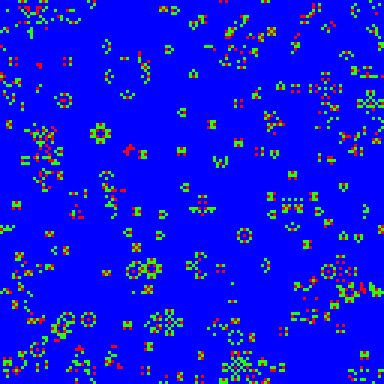
\includegraphics[width=\linewidth]{figures/micro4.png}
  \caption{A \acl{CA} with visible emergent structures.}
  \label{fig:structured_sys}
\end{subfigure}
\caption{Two examples of complex systems (\acf{CA}) with different behavior
  types. Some \acp{CA} appear more promising than others for the design of
  unsupervised learning systems because of their emergent complex structures
  (visible in \ref{fig:structured_sys}), whereas the \ac{CA} in
  \ref{fig:disordered_sys} seems to behave randomly.}
  \label{fig:comparison_ca}
\end{figure}

  \item Measure the fraction of systems that have the most complex and rapidly
        evolving behavior. Defining these notions is also part of the goal. We
        believe those systems to be the most promising for further use since
        they may exhibit open-ended complexity growth. In Chapters
        \ref{cha:meas-compl-evolv} and \ref{cha:visu-comp-large}, we present
        different methods to measure evolving complexity and understand when the
        complexity increases over time. In Chapter \ref{cha:visu-comp-large} we
        study the importance of multi-scale analysis for the complexity of
        cellular automata, and identify complex systems with behavior that
        changes when we scale the system up or down.
\begin{figure}[htbp]
  \centering
 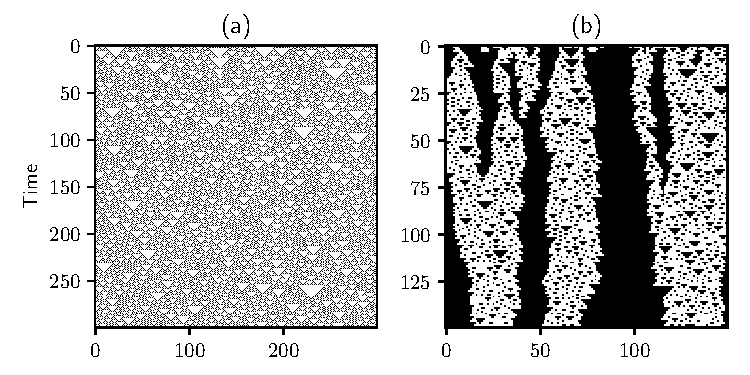
\includegraphics[width=.9\linewidth]{figures/rule18_small}
 \caption{Filtering the behavior of elementary \acl{CA} rule 18. This
   uncovers a highly structured behavior with the propagation of area boundaries
   within the apparent randomness.}
  \label{fig:rule_18}
\end{figure}

  \item Apply promising systems to challenging learning tasks where classical
        machine learning models may fail or prove less efficient. The goal is to
        define various ways to apply evolving complex dynamical systems to some
        standard learning tasks and to figure out if it improves the performance
        or efficiency of the learning algorithm. An example application that we
        explore in Chapter \ref{cha:learn-effic-compl} is illustrated in
        Figure~\ref{fig:ca_lm}, where a \ac{CA} is used to implement a language
        model, a probabilistic model that is used to generate text to complete
        sentences. In Chapter \ref{cha:background}, we explore the similarities
        between \acp{CA} and a special type of neural networks, which highlights
        the numerous potential applications of the former.
\begin{figure}[htbp]
  \centering
  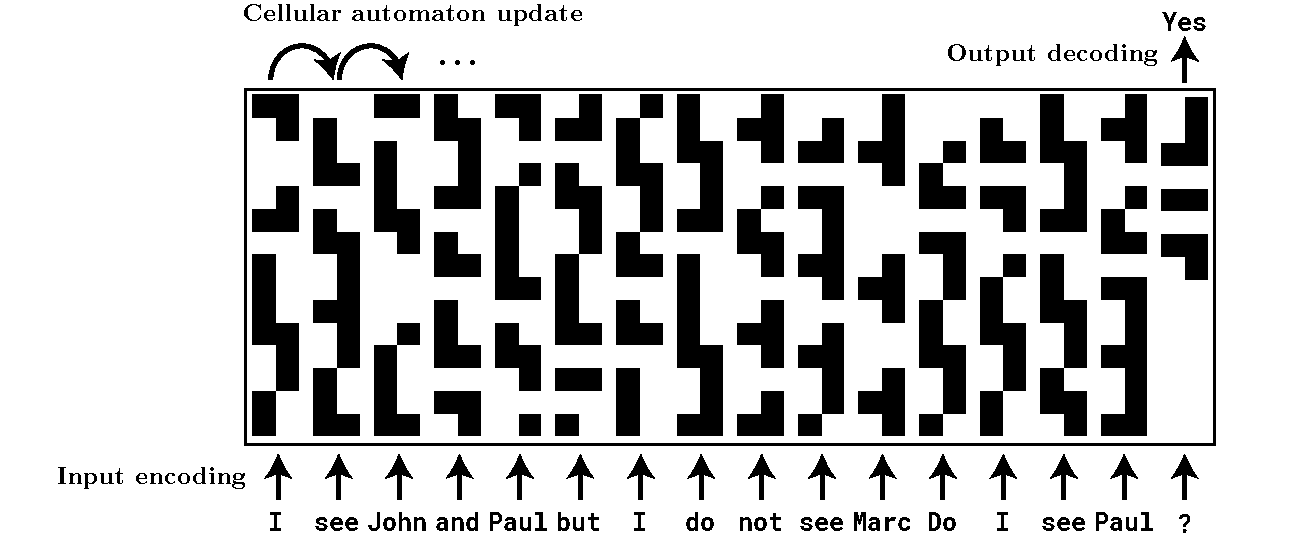
\includegraphics[width=\linewidth]{figures/ca_lm}
  \caption{An example of using a \acl{CA} and reservoir computing to implement a
    language model. Tokens are encoded within the \acl{CA} internal state. The
    \acl{CA} update rule is then applied and an output value is decoded from the
    final state.}
  \label{fig:ca_lm}
\end{figure}

\end{enumerate}

In this thesis, we do not focus our attention on what the machine learning
community commonly refers to as ``unsupervised learning'', that is, learning
structure from untagged data
\parencite{hintonUnsupervisedLearningFoundations1999}. In machine learning,
supervision refers to a label, a number, or a collection of numbers that
represents an expected outcome associated with some input data. Our goal is to
construct models that can develop autonomously, so we first seek systems that
behave in that way on their own and postpone the issue of learning to optimize a
particular objective function. We are particularly interested in systems that
can develop through internal evolution rules, without any input, which is the
case for many complex systems.

We work toward achieving these goals, focusing on one particular complex system:
the \acl{CA}. This model has been extensively studied due to its simple
definition and its ability to simulate a wide range of complex behaviors. We
provide a detailed description of \aclp{CA} in Section
\ref{sec:cellular-automata-sec}. This thesis provides new insights into the role
of learning in complex systems and open-ended evolution, and demonstrates the
potential of cellular automata as a model for studying these phenomena.

\section{Motivation}

It is possible that some form of evolutionary mechanism may be necessary in
order to achieve certain types of AI, particularly if the goal is to create
intelligent systems that can adapt and learn in complex and changing
environments. Complex dynamical systems could be key to overcome the problems
with existing learning algorithms, such as difficulties in generalization,
robustness, or the ability to learn continuously
\parencite{parisiContinualLifelongLearning2019}. The natural intelligence of
biological systems seems to rely on emerging properties selected through
evolution. For example, biological life exhibits a pattern of major evolutionary
transitions where lower-level autonomously replicating entities merge to form a
single more complex corporate body
\parencite{lorenzEmergenceModularityBiological2011}. This is believed to have
occurred for the emergence of eukaryotic cells, as well as for multicellular
life \parencite{hammerschmidtLifeCyclesFitness2014}. All complex and diverse
biological entities have presumably emerged from a single common ancestor and,
even before, from inorganic components present on the surface of the Earth.

So far, it is unclear what algorithmic properties could lead an artificial
system to display a similar trajectory in its state space. Producing emerging
phenomena similar to those of nature \emph{in silico} is a long-standing
challenge. There is a history of algorithms that attempt to apply evolutionary
design to solve particular tasks, called evolutionary algorithms
\parencite{fogelArtificialIntelligenceSimulated1966,
  ,millerDesigningNeuralNetworks1989, backOverviewEvolutionaryAlgorithms1993}.
However, many of these methods focus on searching the space of solutions using
high-level evolutionary mechanisms, such as genetic mutations and crossovers.
Although effective in solving precise tasks, these methods often obscure another
crucial component of natural evolution by using an explicit fitness function.

Most existing machine learning algorithms rely on the choice of an objective
function: a clearly defined mapping from the current state and parameters of a
model to a real value, which indicates the performance of that model. The
function depends on the objective of the model. For a supervised learning
problem, we may count the number of misclassified objects or the distance between
the predictions and the expected results. Even in unsupervised learning, the family of
algorithms learning from untagged data, objectives are still used. For
example, the well-known K-means clustering algorithm minimizes the sum of square
distances to cluster centers.

This reliance on objective functions creates two main issues: (i) the objective
is not always clearly defined or can be too broad for general-purpose
applications. For example, a possible objective function for a walking robot
could be to ``not fall when stepping through its surrounding environment''. This
function is impractical to define and will vary greatly depending on the
parameters of the environment. Furthermore, (ii) using such functions as goals
can be counterproductive because, as many examples in nature demonstrate, robust
paths to complex objectives are often deceptive. They involve developing in
unexpected directions that may initially seem against the original goal
\parencite{stanleyWhyGreatnessCannot2015}.

In this thesis, the term \emph{unsupervised} refers to a form of learning with
no predefined objective. Like in natural evolution, we expect unsupervised
algorithms to develop new features autonomously and become progressively more
complex over time. Such algorithms would regularly learn to solve problems on
their own without the need to explicitly guide them, thereby discovering robust
and diverse solutions to deceptive problems.


\section{Challenges}\label{sec:challenges}

\begin{figure}[htbp]
  \centering
  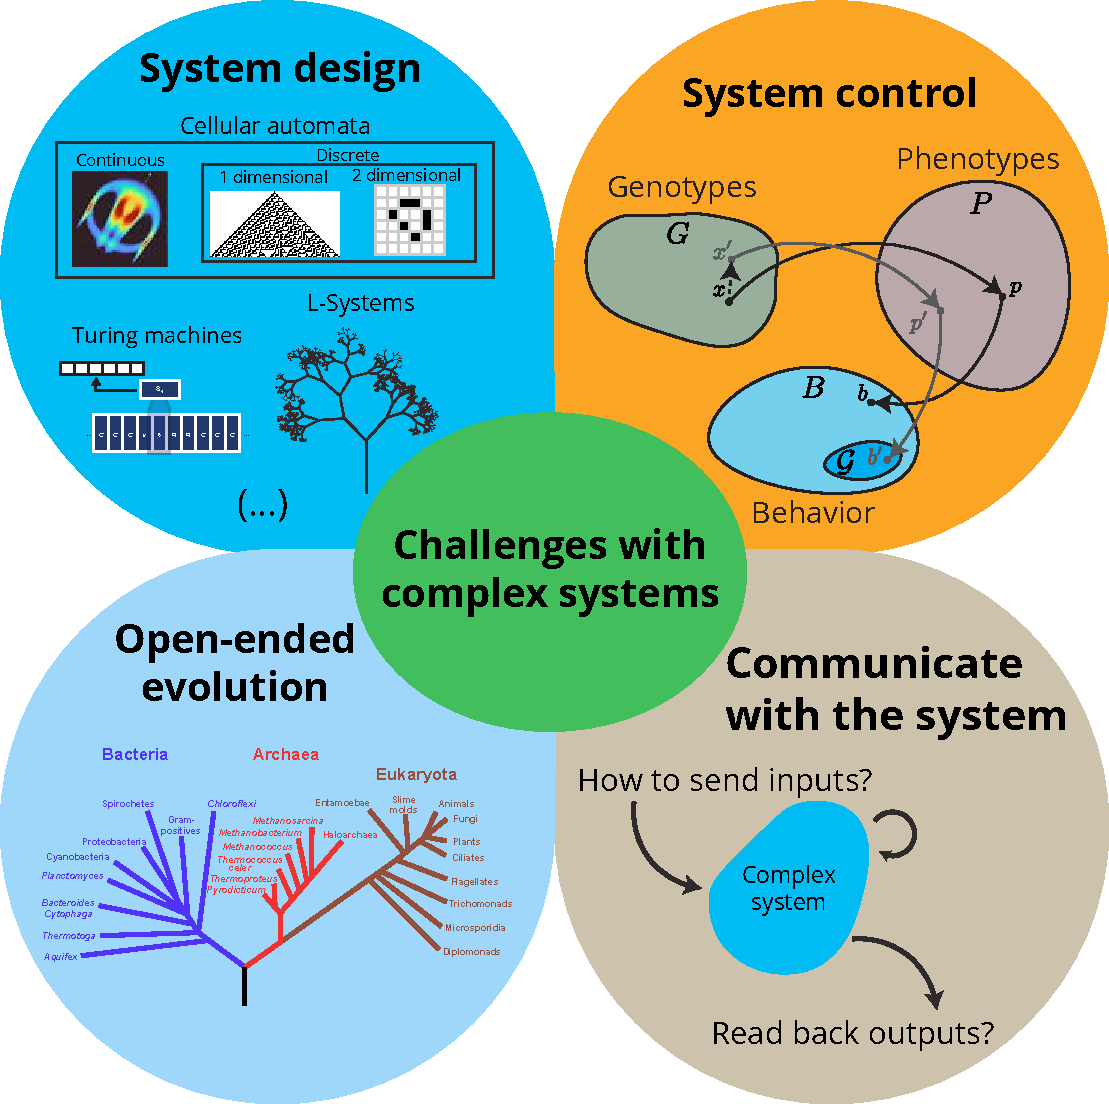
\includegraphics[width=.98\linewidth]{figures/challenges}
  \caption{The challenges of working with complex systems encountered across
    this thesis can be broken down in several categories. (top-left) The choice
    and design of the system, (top-right) the control of the system which
    involves understanding the complex mapping between a parameter space and the
    possibly unpredictable behavior of a system, (bottom-left) the search for
    open-ended evolution properties similar to the ones found in nature,
    (bottom-right) the issue of sending inputs and reading outputs from the
    internal state of a complex system. This illustration uses
    \href{https://commons.wikimedia.org/wiki/File:Lenia_icon4.png}{Lenia
      icon4.png} by Bert Wang-Chak Chan, licensed under
    \href{https://creativecommons.org/licenses/by-sa/4.0/}{CC BY 4.0}. }
  \label{fig:challenges}
\end{figure}

The study of complex systems poses a range of difficult challenges in and of
itself \parencite{sanmiguelChallengesComplexSystems2012}. The complexity of a
system is an emergent property that arises from its intricate structure, its
number of elements, how it functions, and how it responds to different kinds of
external influence. For many complex systems, their emergent mechanisms are
poorly understood. We identify four main challenges associated with the study of
complex systems: the questions of the design choices in defining and sampling a
complex system (section \ref{sec:design-compl-syst}), which will in turn define
their potential for supporting a form open-ended evolution (section
\ref{sec:open-ended-evolution}) and how we can expect to build an interface to
communicate with it (section \ref{sec:compl-syst-inputs}), which is essential to
achieve some for of control of that system (section \ref{sec:compl-syst-contr}).

\subsection{Design of a complex system\label{sec:design-compl-syst}}

The definition of complex systems is broad, and several systems with interesting
dynamics have been studied. For example, L-Systems, Random Boolean networks,
Turing machines, and \Acfp{CA}. In this thesis, we focus mainly on the latter:
\acl{CA}. There are multiple benefits to working with this model. It is very
simply defined, and its high parallelism makes its implementation
straightforward. Moreover, \acp{CA} have demonstrated an ability to simulate a
wide range of complex behaviors \parencite{wolframNewKindScience2002}.

Choosing the right complex system architecture is essential because it defines
the search space over which interesting and useful systems can be found.
Correctly parameterizing that space can also be challenging, because too many
degrees of freedom make it difficult to search for and find good systems, while
too few might indicate a lack of expressivity. An example parameterization of
\ac{CA} with little expressivity is Langton's lambda parameter
\parencite{langtonComputationEdgeChaos1990}. At the other end of the spectrum, the
\ac{CA} rule is a simple parametrization with many degrees of freedom, which
makes it impractical.

Even when we limit ourselves to the study of \ac{CA}, many variants can be
considered. Cellular automata can have continuous or discrete states and operate
in continuous or discrete space. For discrete state and space cellular automata,
the number of states and window of the update function can vary, as well as the
topology of the simulation space. We tackle this issue from various angles
across the thesis, exploring the question of rule definition in Chapter
\ref{cha:meas-compl-evolv}, the scale in Chapter \ref{cha:visu-comp-large} and
the connectivity pattern in Chapter \ref{cha:learn-effic-compl}.

\subsection{Complex systems control}\label{sec:compl-syst-contr}

\begin{figure}[htbp]
  \centering
  \begin{subfigure}[t]{.47\linewidth}
    \centering
    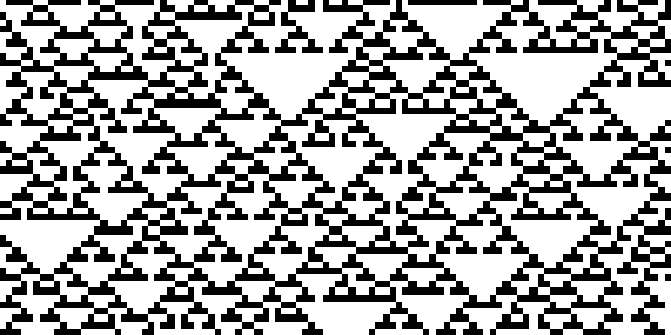
\includegraphics[width=.93\linewidth]{figures/ca_comp_a}
    \caption{\ac{CA} rule 22 on a tape of size 100, ran for 50 steps from a
      random initial state.}
    \label{fig:ca_comp_a}
  \end{subfigure}
  \hspace{10pt}
  \begin{subfigure}[t]{.47\linewidth}
    \centering
    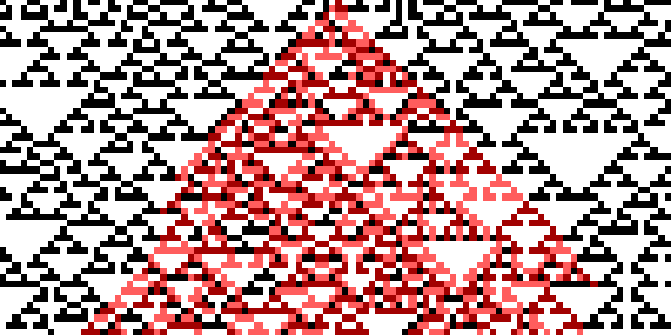
\includegraphics[width=.93\linewidth]{figures/ca_comp_b}
    \caption{\ac{CA} rule 22 on a tape of size 100, ran from a slightly
      different initial state. The cells different from Figure \ref{fig:ca_comp_a} are
      overlayed in red.}
    \label{fig:ca_comp_b}
  \end{subfigure}

  \caption{Comparison of the same 1 dimensional \ac{CA} ran from two initial conditions
    differing only by one cell. Each row is the state of the \ac{CA} at one time
    step. The effect of the small perturbation of initial conditions grows
    rapidly as the \ac{CA} evolves in time.}
  \label{fig:ca_comp}
\end{figure}


Even if we want complex systems that evolve in unexpected directions and grow in
an open-ended way without supervision, it may still be useful to steer them
locally towards specific targets. A major challenge that follows from this goal
is that many complex systems are chaotic. A deterministic dynamical system is
said to be chaotic if its evolution is highly sensitive to its initial
conditions. Because of this property, it is often very hard to predict how a
given system will evolve over time, and therefore hard to steer its evolution
towards a particular final state or along a chosen trajectory. This is an
advantage for creating open-ended systems, but it can be challenging to apply
these systems to some basic tasks.

This problem is also related to the issue of sending a control signal to a
complex system, which depends on a choice of encoding.

\subsection{Complex systems inputs and outputs\label{sec:compl-syst-inputs}}

Some of the complex systems we study in this thesis are closed systems. They do
not expect inputs or have any well-defined outputs. For example, \ac{CA} and
\ac{RBN} do not have a notion of inputs and outputs built into the model. They
are standalone objects that evolve according to a set of internal rules.

A common challenge for such systems is to define the inputs and outputs in a way
that preserves their internal dynamics. This is also connected to the control
problem of Section \ref{sec:compl-syst-contr}, because controlling a complex
system implies being able to send a control signal and read back its current
state.

Throughout this work, we use reservoir computing for this purpose. Reservoir
computing allows one to harvest the internal computations of complex systems, or
\emph{read} information from its internal state by learning a linear regression
that maps that internal state to desired outputs (see Section
\ref{sec:res-models}).



\subsection{Open-ended evolution without
  objectives}\label{sec:open-ended-evolution}

Another challenge is posed by the absence of a clear objective in the design of
unsupervised learning systems. Even without an objective, it is still essential
to understand which complex systems to choose from all available options or how
to tune their parameters so that they behave in interesting ways. For example,
\acp{CA} such as the one showed in Figure \ref{fig:disordered_sys} are not
likely to be useful for construction systems that exhibit growth of complexity.

This is why we need metrics that can help select systems without being another
replacement objective function. Our goal is to create a system that has the
property of evolving in an open-ended way. We address this challenge in
particular in Chapter~\ref{cha:meas-compl-evolv}, by designing a complexity
metric that can help select interesting complex systems, without relying on some
task-based performance score.

\section{Contributions}

The main contributions of this thesis are as follows.
\begin{enumerate}
  \item A literature review making the connection between cellular automata and
        other complex systems, open-ended evolution and neural networks.
        Studying these fields from a single point of view is relatively novel,
        and we consider a review necessary for placing the rest of our work in
        its context.

  \item The development of a general complexity metric that can help identify
        complex systems with interesting behavior.

  \item Development of a coarse-graining method to visualize computations
        in cellular automata and other discrete systems with local interactions.

  \item The introduction of a metric for learning efficiency for learning
        algorithms as well as a benchmark dataset of progressively harder
        language tasks.
\end{enumerate}

\section{Thesis overview}

In Chapter \ref{cha:literature-review}, we review relevant methods and tools for
measuring the complexity of complex systems and using their computations for
various tasks.

Chapter \ref{cha:background} presents some background notions about complex
systems, cellular automata, and reservoir computing.

Chapter \ref{cha:meas-compl-evolv} introduces a complexity metric that allows us 
to select complex systems with interesting behavior. The metric measures the
``novelty'' of the temporal states of a system compared to a reference one. We
built a dataset of interesting cellular automata to validate the quality of the
metric.

Chapter \ref{cha:visu-comp-large} addresses the question of large-scale complex
systems and the applicability of complexity metrics at multiple scales. We
propose three algorithms for the coarse-graining of cellular automata. This allows
us to reduce the size of large-scale systems while retaining the interesting parts
of the behavior.

Chapter \ref{cha:learn-effic-compl} presents a learning efficiency metric and a
dataset to measure the speed of learning of various systems. We show that
reservoir computing-based systems using cellular automata can be more efficient
than usual machine learning algorithms in constrained data and computation
settings.

\section{Publications and software}

The thesis has led to the following publications.

\begin{itemize}
  \item \fullcite{cisnerosEvolvingStructuresComplex2019}
  \item \fullcite{cisnerosVisualizingComputationLargescale2020}
  \item \fullcite{cisnerosBenchmarkingLearningEfficiency2022}
\end{itemize}

The code to reproduce the experiments of all three publications is available on
GitHub. We also published a dataset that we used for our benchmark in our last
publication. It is available at
\url{https://github.com/hugcis/incremental_tasks/}.
